\documentclass[pl]{aghdpl}
\usepackage[polish]{babel}

% dodatkowe pakiety
\usepackage{float}
\usepackage{pgffor}
\usepackage{enumerate}
\usepackage{listings}
\usepackage[T1]{fontenc}
\usepackage[utf8]{inputenc}
\usepackage{enumitem}
\usepackage{tocloft}
\usepackage{mcode}
\lstloadlanguages{TeX}

\renewcommand{\thefigure}{\thesection.\arabic{figure}}
\renewcommand{\thetable}{\thesection.\arabic{table}}
\renewcommand{\cftloftitlefont}{\Large\bfseries}

\makeatletter
\@openrightfalse
\DeclareRobustCommand{\em}{%
	\@nomath\em \if b\expandafter\@car\f@series\@nil
	\normalfont \else \bfseries \fi}
\makeatother

\lstset{
	literate={ą}{{\k{a}}}1
	{ć}{{\'c}}1
	{ę}{{\k{e}}}1
	{ó}{{\'o}}1
	{ń}{{\'n}}1
	{ł}{{\l{}}}1
	{ś}{{\'s}}1
	{ź}{{\'z}}1
	{ż}{{\.z}}1
	{Ą}{{\k{A}}}1
	{Ć}{{\'C}}1
	{Ę}{{\k{E}}}1
	{Ó}{{\'O}}1
	{Ń}{{\'N}}1
	{Ł}{{\L{}}}1
	{Ś}{{\'S}}1
	{Ź}{{\'Z}}1
	{Ż}{{\.Z}}1
}
%---------------------------------------------------------------------------------------------------
\author{Miłosz Mach}
\shortauthor{M.Mach}

\titlePL{Analiza regulatorów strojonych metodami automatycznego strojenia zaimplementowanymi w Matlab Control Toolbox dla pierwszego zestawu problemów}
\titleEN{Analysis of regulators tuned automatically by tools implemented in Matlab Control Toolbox for the first set of problems}

\shorttitlePL{Analiza regulatorów strojonych metodami automatycznego strojenia zaimplementowanymi w Matlab Control Toolbox dla pierwszego zestawu problemów}
\shorttitleEN{Analysis of regulators tuned automatically by tools implemented in Matlab Control Toolbox for the first set of problems}

\thesistype{Projekt}

\supervisor{Jerzy Baranowski, dr inż.}

\degreeprogramme{AiR, Komputerowe Systemy Sterowania, Robotyka}

\date{2016}

\department{Katedra Automatyki i Inżynierii Biomedycznej}

\faculty{Wydział Elektrotechniki, Automatyki,\protect\\[-1mm] Informatyki i Inżynierii Biomedycznej}

 \acknowledgements{}

%---------------------------------------------------------------------------------------------------
\begin{document}

\titlepages
\setcounter{tocdepth}{3}
\tableofcontents

\chapter*{Wstęp}
\addcontentsline{toc}{chapter}{Wstęp}

Celem niniejszego projektu jest analiza regulatorów strojonych automatycznie przy wykorzystaniu  narzędzi zaimplementowanych w pakiecie Matlab Control Toolbox. W pierwszej kolejności autor opisuje 3 różne podejścia do tematu automatycznego strojenia regulatorów. Następnie, po wybraniu narzędzia zapewniającego najlepszą możliwość automatyzacji procesu, przedstawia wyniki strojeń wszystkich 134 obiektów.
\chapter{Wprowadzenie teoretyczne}
\label{cha:wteoretyczny}
Matlab Control Toolbox to przybornik dostarczający narzędzia i algorytmy do analizy, projektowania oraz strojenia liniowych układów regulacji. Umożliwia pracę na układach reprezentowanych przykładowo przez transmitancje (transfer function) oraz równania stanu (state-space).Pozwala analizować zachowanie układu w dziedzinie czasowej oraz częstotliwościowej. W szczególności, przybornik posiada zestaw narzędzi służących do strojenia regulatorów PID tak, by regulowany układ w satysfakcjonującym czasie osiągnął wartość zadaną, możliwie bez przeregulowań.

\section{PID Tuner}
\label{sec:wpr_pidtune}
Pierwszym rozwiązaniem jest skorzystanie z automatycznej, interaktywnej metody  strojenia regulatorów PID dla systemów SISO. Dostęp do niej uzyskuje się poprzez umieszczenie w modelu Simulink bloczka PID, a następnie wybranie opcji Tune widocznej przy parametrach regulatora.
Można również skorzystać z komendy

\textit{pidTuner(sys,type)}.

\begin{figure}[H]
	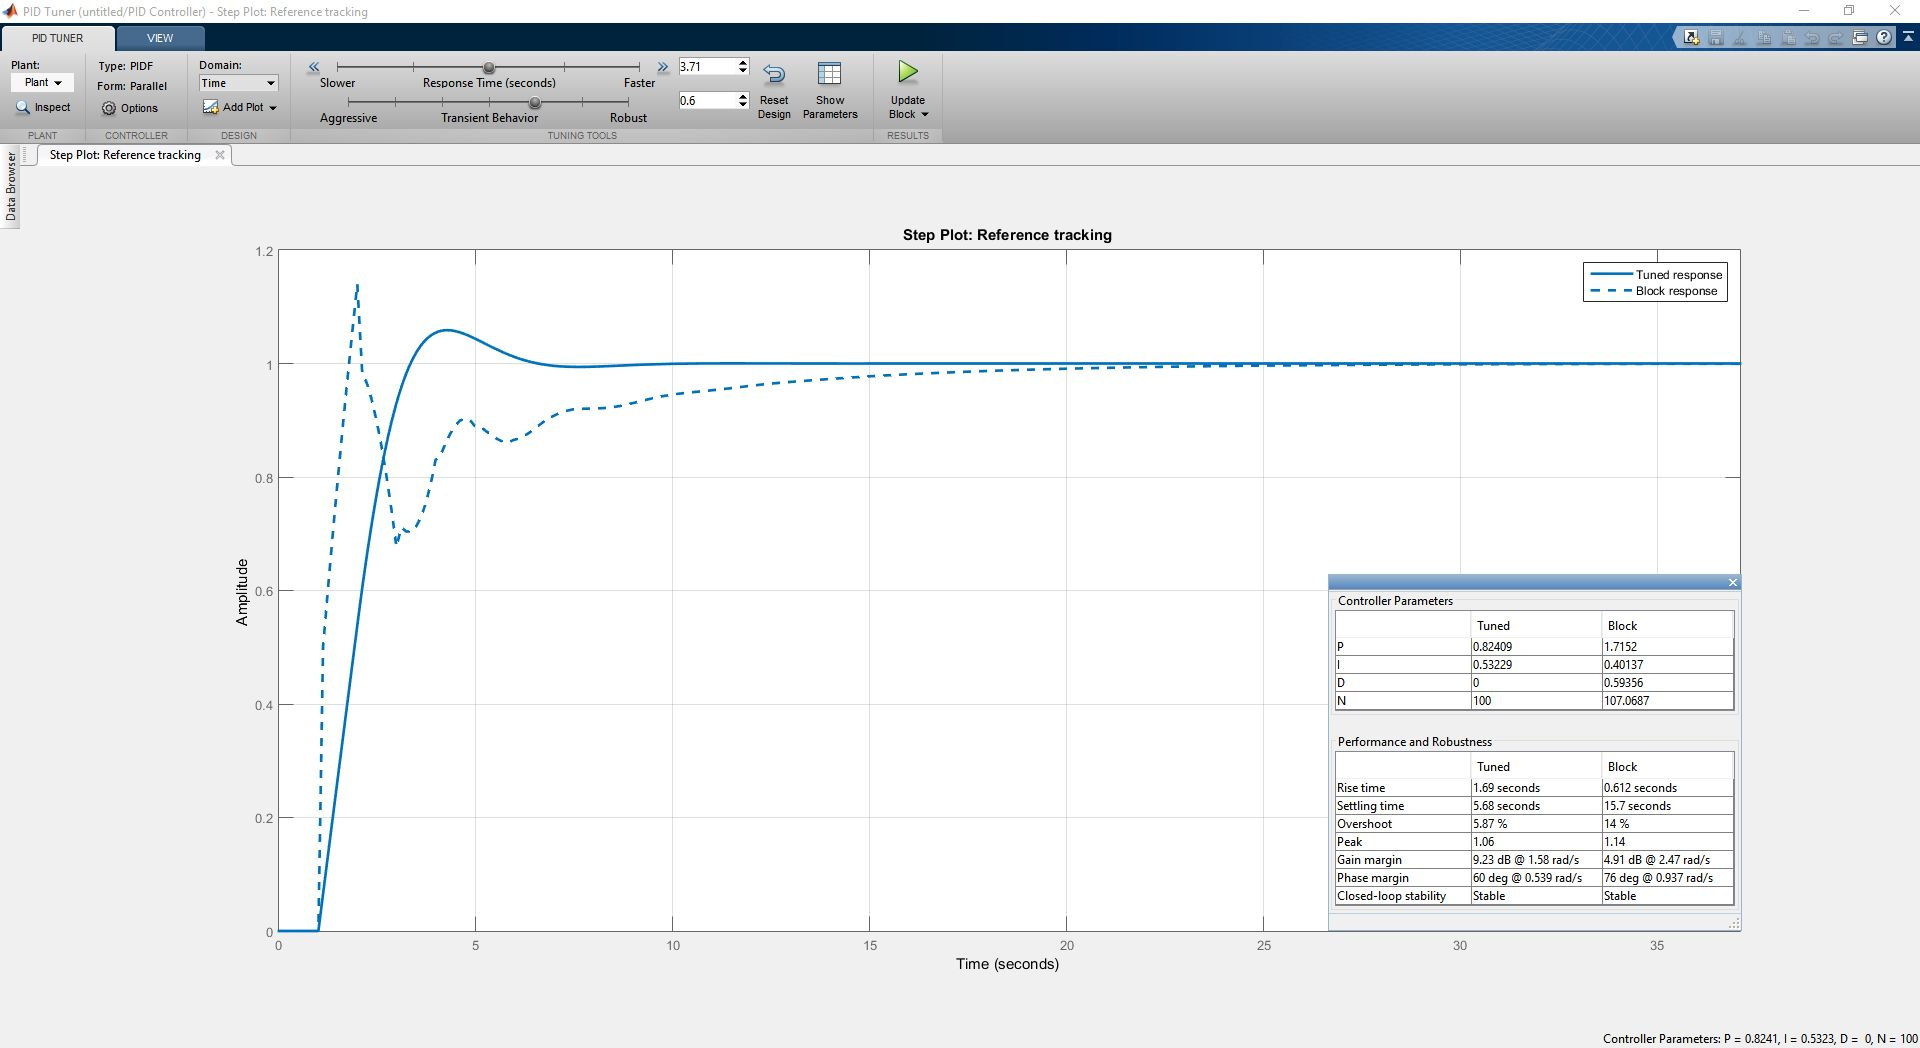
\includegraphics[width=160mm]{PID_Tuner}
	\caption{Zrzut ekranu przedstawiający narzędzie PID Tuner}
	\label{fig:PID_Tuner}
\end{figure}

\noindent Otwiera się wówczas okno, które bazując na podanym modelu wyświetla jego aktualną odpowiedź. Użytkownik jest w stanie zmienić typ regulatora, domyślnie pozostając przy PID. Korzystając z suwaków, można modyfikować czas reakcji oraz agresywność odpowiedzi. Podczas takich zmian, użytkownik na bieżąco obserwuje odpowiedź układu oraz zmieniające się parametry regulatora.
Możliwe jest również wyświetlenie innych przebiegów - takich, jak odpowiedź układu otwartego, odpowiedź skokowa obiektu regulacji - w dziedzinie czasowej lub częstotliwościowej.




\section{SISO Design Tool}
\label{sec:wpr_pidtune}
Kolejne narzędzie do tworzenia regulatorów i filtrów wejściowych dla
układów o jednym wejściu i jednym wyjściu. Program posiada wygodny interfejs umożliwiający bieżący podgląd charakterystyk czasowych i częstotliwościowych
zarówno układu otwartego (dla regulatora) oraz zamkniętego (obiekt + regulator). Użytkownik definiuje układ poprzez wybór jednego ze schematów, podaje wartości obiektów (np. z Workspace'a), a następnie przechodzi do zakładki poświęconej strojeniu.
Narzędzie uruchamia się poprzez wpisanie komendy

\textit{controlSystemDesigner}.

\begin{figure}[H]
	\centering
	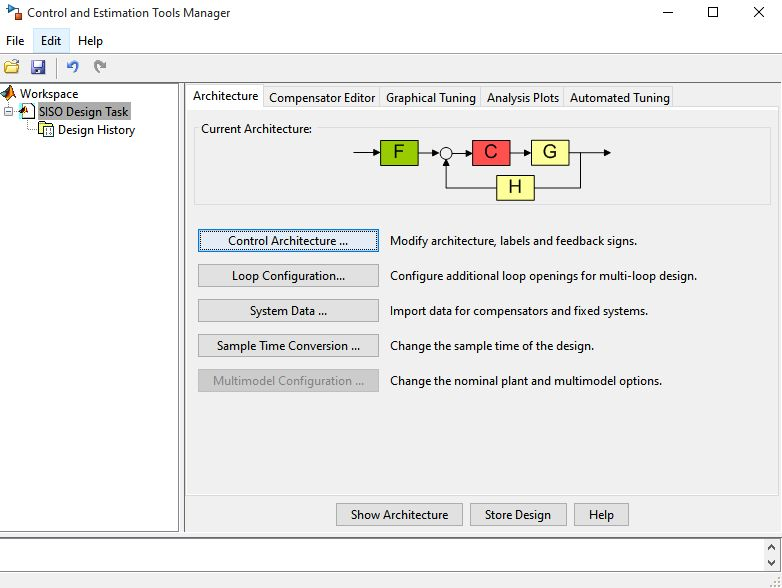
\includegraphics[width=130mm]{SISO_Design_Tool1}
	\caption{Zrzut ekranu przedstawiający narzędzie definiowanie obiektu w SISO Design Tool}
	\label{fig:SISO_Design_Tool1}
\end{figure}
\begin{figure}[H]
	\centering
	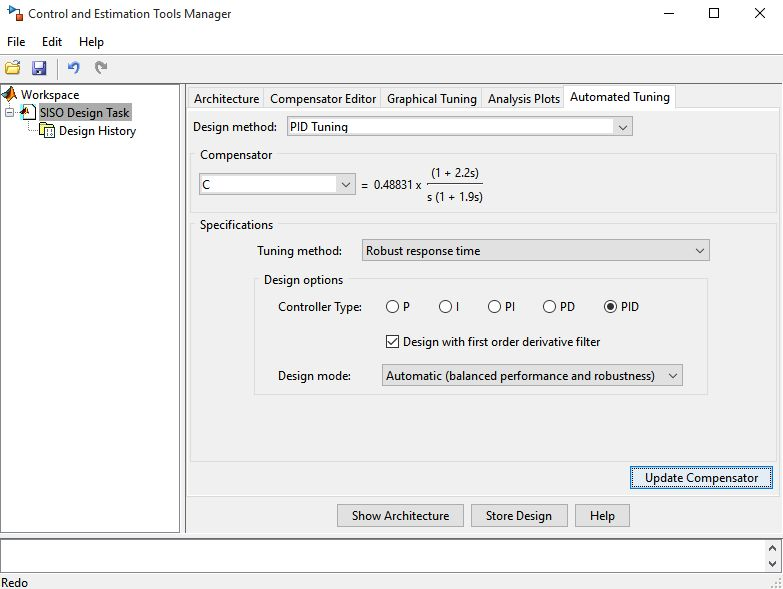
\includegraphics[width=130mm]{SISO_Design_Tool2}
	\caption{Zrzut ekranu przedstawiający proces automatycznego strojenia w SISO Design Tool}
	\label{fig:SISO_Design_Tool2}
\end{figure}





\section{Strojenie z wiersza poleceń}
\label{sec:wpr_Command_Line_Tuning}
Ostatnim i zarazem wykorzystanym w niniejszym projekcie sposobem jest strojenie regulatora za pomocą komendy uruchamianej w skrypcie. Umożliwiło to automatyzację działań. Polecenie

\textit{pidTune(sys,type,opts)}.

\noindent zaprojektuje regulator typu \textit{type} dla obiektu \textit{sys} w pętli sprzężenia zwrotnego. Funkcja zwraca  obiekt \textit{pid} oraz informacje na temat:
\begin{itemize}
	\item Stabilności,
	\item Częstotliwości crossover,
	\item Zapas fazy.
\end{itemize}
Komenda pozwala dodać opcje modyfikujące  domyślne ustawienia strojenia. Są to:
\begin{itemize}
	\item Zapas fazy (domyślnie 60),
	\item Tryb strojenia (domyślnie \textit{balanced}),
	\item Ilość niestabilnych pierwiastków.
\end{itemize}
\chapter{Rozwiązanie}
\label{cha:rozw}

\section{Wst\k{e}p}
\label{sec:rozw_wstep}
Celem projektu jest nastrojenie regulatorów dla następujących procesów:
 \begin{itemize}

	 \item $ P_{1}(s) = \frac{e^{-s}}{1 +sT}	$,
	
	gdzie T = 0.02, 0.05, 0.1, 0.2, 0.3, 0.5, 0.7, 1, 1.2, 1.5, 2, 4, 6, 8, 10, 20, 50, 100, 200, 500, 1000

	\item $ P_{2}(s) = \frac{e^{-s}}{(1 +sT)^2} $,
	
	gdzie T = 0.01, 0.02, 0.05, 0.1, 0.2, 0.3, 0.5, 0.7, 1, 1.2, 1.5, 2, 4, 6, 8, 10, 20, 50, 100, 200, 500
	
	\item $ P_{3}(s) = \frac{e^{-s}}{(1 +s)(1 +sT)^2}	$,
	
	gdzie T = 0.005, 0.01, 0.02, 0.05, 0.1, 0.2,  0.5,  2, 5, 10
	
	\item $ P_{4}(s) = \frac{1}{(1 +s)^n}	$,
	
	gdzie n =3, 4, 5, 6, 7, 8
	
	\item $ P_{5}(s) = \frac{1}{(1 +s)(1 +\alpha s)(1 +\alpha^2 s)(1 +\alpha^3s)}	$,
	
	gdzie \(\alpha \) = 0.1, 0.2, 0.3, 0.4, 0.5, 0.6, 0.7, 0.8, 0.9
	
	\item $ P_{6}(s) = \frac{e^{-sL}}{s(1 +sT)} $,
	
	gdzie L = 0.01, 0.02, 0.05, 0.1, 0.3, 0.5, 0.7, 1 i 
	T + L = 1
	
	\item $ P_{7}(s) = \frac{Te^{-sL}}{(1 +sT)(1 +sT1)} $,
	
	gdzie T = 1, 2, 5, 10 i 
	L = 0.01, 0.02, 0.05, 0.1, 0.3, 0.5, 0.7, 1 i 
	T1 + L = 1
	
	\item $ P_{8}(s) = \frac{1 - \alpha s}{(s+1)^3} $,
	
	gdzie \(\alpha \) = 0.1, 0.2, 0.3, 0.4, 0.5, 0.6, 0.7, 0.8, 0.9, 1, 1.1
	
	\item $ P_{8}(s) = \frac{1}{(s+1)((sT)^2 + 1.4sT + 1)}	$,
	
	gdzie T = 0.1, 0.2, 0.3, 0.4, 0.5, 0.6, 0.7, 0.8, 0.9, 1
 	
 \end{itemize}
Po wprowadzeniu i posegregowaniu każdej transformaty w Matlabie, utworzono przedstawiony w następnej sekcji skrypt, którego zadaniem jest zautomatyzowane obsłużenie każdego obiektu. Obsługa ta zakłada:

\begin{itemize}
	\item Wyrysowanie odpowiedzi skokowej obiektu;
	\item Zaprojektowanie regulatora PID;
	\item Wyrysowanie przebiegów na podstawie modelu, który w pierwszej sekundzie symulacji zmienia wartość zadaną z 0 na 1:
	\begin{itemize}
		\item[$\bullet$] bez modyfikowanego sterowania,
		\item[$\bullet$] ze sterowaniem poddanym saturacji,
		\item[$\bullet$] ze sterowaniem poddanym saturacji oraz szumem na wartości zadanej oraz wyjściu obiektu.
	\end{itemize}
\end{itemize}




\section{Źródła}
\label{sec:zrodla}
\begin{figure}[H]
<<<<<<< HEAD
	\centering
=======
>>>>>>> origin/master
	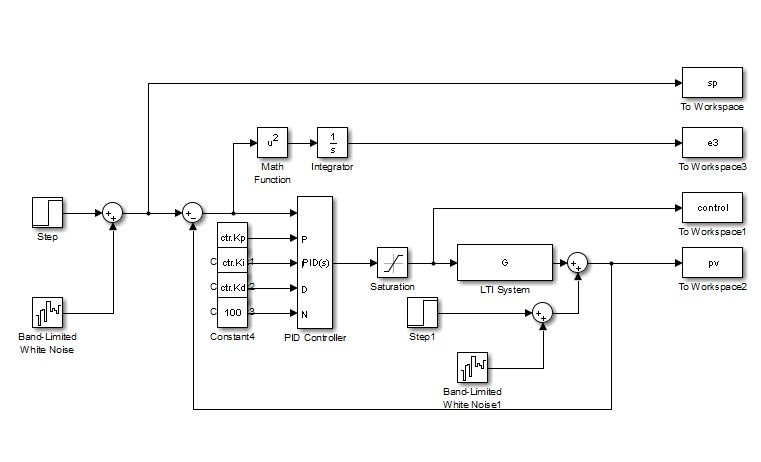
\includegraphics[width=140mm]{ClosedLoopModel.jpg}
	\caption{Model w Simulinku}
	\label{fig:model_simulink}
\end{figure}

Poniżej przedstawiono skrypt napisany w Matlabie.
\begin{lstlisting} 
quality=[];
load('transfer_functions.mat')
n=9;
m=[21 21 10 6 9 9 36 11 10];
simulation_time = 30;
model_nsat = 'PIDmodel_nsat.slx';
model_sat = 'PIDmodel_sat.slx';
model_sat_noise = 'PIDmodel_sat_noise.slx';
for i = 1:n
	for j=1:m(i)
		try
			%% Load transfer function %%
			name=strcat('G',num2str(i),'(',num2str(j),')');
			G = eval(name);
			transfer_function=strcat('$$G(s)=',latex(poly2sym(cell2mat(eval(strcat(name,'.num'))),s)
				/poly2sym(cell2mat(eval(strcat(name,'.den'))),s)),'$$');
		
			%% Plot step response %%
			fig = figure();
			h=subplot(2,1,1);
			step(G,simulation_time);
			grid on;
		
			%% Design PID controller %%
			[ctr,info]=pidtune(G,'pid');
			cmd_sys=feedback(ctr*G,1);    
		
			%% Perform simulation (not saturated), plot model response %%
			sim(model_nsat); 
			
			h=subplot(2,1,2);
			plot(sp, 'r');
			hold on;
			plot(control, 'g');
			plot(pv, 'b');
			grid on;
			ylabel('Amplitude');
			xlabel('Time (seconds)');
			title(strcat(transfer_function,', Saturation: off, Noise: off', ', e=',
			num2str(e1.Data(length(e1.Data)))), 'Interpreter', 'Latex')
			legend('set value','control value','response value', 'Location','southeast');
		
			%% Save to file 1%%
			file = strcat('sprawozdanie\G',int2str(i),'-tf-', int2str(j),'a');
			print(fig,file,'-dpng');
			close(fig)
			%% Perform simulation (saturated), plot model response %%
			sim(model_sat); 
	
			fig = figure();            
			h=subplot(2,1,1);
			plot(sp, 'r');
			hold on;
			plot(control, 'g');
			plot(pv, 'b');
			grid on;
			ylabel('Amplitude');
			xlabel('Time (seconds)');
			title(strcat(transfer_function, ', Saturation: on, Noise: off ',',
			 e=',num2str(e2.Data(length(e2.Data)))), 'Interpreter', 'Latex')
			legend('set value','control value','response value', 'Location','southeast');
	
	
	
			%% Perform simulation (saturated with noise), plot model response %%
			sim(model_sat_noise);
		
			h=subplot(2,1,2);
			plot(sp, 'r');
			hold on;
			plot(control, 'g');
			plot(pv, 'b');
			grid on;
			ylabel('Amplitude');
			xlabel('Time (seconds)');
			title(strcat(transfer_function, ', Saturation: on, Noise: on ',',
			 e=',num2str(e3.Data(length(e3.Data)))), 'Interpreter', 'Latex')
			legend('set value','control value','response value', 'Location','southeast');
	
			quality=[quality; i j e1.Data(length(e1.Data)) e2.Data(length(e2.Data)) e3.Data(length(e3.Data))];
			%% Save to file 2%%
			file = strcat('sprawozdanie\G',int2str(i),'-tf-', int2str(j),'b');
			print(fig,file,'-dpng');
			close(fig)
		catch ME
			strcat('Błąd w: G',int2str(i),'(',int2str(j),').')
		end
	end
end
save('sprawozdanie\report.txt','quality','-ascii')

\end{lstlisting}



\section{Analiza układu zamkniętego}
\label{sec:zamkniety}
<<<<<<< HEAD
Należy zwrócić uwagę, iż każda poniższa strona poświęcona jest innemu obiektowi. W sprawnej nawigacji po tym rozdziale może pomóc spis rysunków dostępny na końcu pracy.
=======
>>>>>>> origin/master
\foreach \y in {1,...,21}{
	\begin{figure}[H]
		\centering
		\includegraphics[width=140mm]{G1-tf-\y a}
		\caption{Obiekt G1-tf\y a}
		\label{fig:G1-tf-\y a}
	\end{figure}
	\begin{figure}[H]
		\centering
		\includegraphics[width=140mm]{G1-tf-\y b}
		\caption{Obiekt G1-tf\y b}
		\label{fig:G1-tf-\y b}
	\end{figure}
}

\foreach \y in {1,...,21}{
	\begin{figure}[H]
		\centering
		\includegraphics[width=140mm]{G2-tf-\y a}
		\caption{Obiekt G2-tf\y a}
		\label{fig:G2-tf-\y a}
	\end{figure}
	\begin{figure}[H]
		\centering
		\includegraphics[width=140mm]{G2-tf-\y b}
		\caption{Obiekt G2-tf\y b}
		\label{fig:G2-tf-\y b}
	\end{figure}	
}

\foreach \y in {1,...,10}{
	\begin{figure}[H]
		\centering
		\includegraphics[width=140mm]{G3-tf-\y a}
		\caption{Obiekt G3-tf\y a}
		\label{fig:G3-tf-\y a}
	\end{figure}
	\begin{figure}[H]
		\centering
		\includegraphics[width=140mm]{G3-tf-\y b}
		\caption{Obiekt G3-tf\y b}
		\label{fig:G3-tf-\y b}
	\end{figure}
}

\foreach \y in {1,...,6}{
	\begin{figure}[H]
		\centering
		\includegraphics[width=140mm]{G4-tf-\y a}
		\caption{Obiekt G4-tf\y a}
		\label{fig:G4-tf-\y a}
	\end{figure}
	\begin{figure}[H]
		\centering
		\includegraphics[width=140mm]{G4-tf-\y b}
		\caption{Obiekt G4-tf\y b}
		\label{fig:G4-tf-\y b}
	\end{figure}
}
\foreach \y in {1,...,9}{
	\begin{figure}[H]
		\centering
		\includegraphics[width=140mm]{G5-tf-\y a}
		\caption{Obiekt G5-tf\y a}
		\label{fig:G5-tf-\y a}
	\end{figure}
	\begin{figure}[H]
		\centering
		\includegraphics[width=140mm]{G5-tf-\y b}
		\caption{Obiekt G5-tf\y b}
		\label{fig:G5-tf-\y b}
	\end{figure}
}
\foreach \y in {1,...,9}{
	\begin{figure}[H]
		\centering
		\includegraphics[width=140mm]{G6-tf-\y a}
		\caption{Obiekt G6-tf\y a}
		\label{fig:G6-tf-\y a}
	\end{figure}
	\begin{figure}[H]
		\centering
		\includegraphics[width=140mm]{G6-tf-\y b}
		\caption{Obiekt G6-tf\y b}
		\label{fig:G6-tf-\y b}
	\end{figure}
}
\foreach \y in {1,...,36}{
	\begin{figure}[H]
		\centering
		\includegraphics[width=140mm]{G7-tf-\y a}
		\caption{Obiekt G7-tf\y a}
		\label{fig:G7-tf-\y a}
	\end{figure}
	\begin{figure}[H]
		\centering
		\includegraphics[width=140mm]{G7-tf-\y b}
		\caption{Obiekt G7-tf\y b}
		\label{fig:G7-tf-\y b}
	\end{figure}
}
\foreach \y in {1,...,11}{
	\begin{figure}[H]
		\centering
		\includegraphics[width=140mm]{G8-tf-\y a}
		\caption{Obiekt G8-tf\y a}
		\label{fig:G8-tf-\y a}
	\end{figure}
	\begin{figure}[H]
		\centering
		\includegraphics[width=140mm]{G8-tf-\y b}
		\caption{Obiekt G8-tf\y b}
		\label{fig:G8-tf-\y b}
	\end{figure}
}
\foreach \y in {1,...,10}{
	\begin{figure}[H]
		\centering
		\includegraphics[width=140mm]{G9-tf-\y a}
		\caption{Obiekt G9-tf\y a}
		\label{fig:G9-tf-\y a}
	\end{figure}
	\begin{figure}[H]
		\centering
		\includegraphics[width=140mm]{G9-tf-\y b}
		\caption{Obiekt G9-tf\y b}
		\label{fig:G9-tf-\y b}
	\end{figure}
}

\chapter{Analiza wyników}
\label{cha:rozw}
 
 Powyżej przedstawiono wykresy stworzone w oparciu o sterowane obiekty. Należy zwrócić uwagę, że przy niektórych transmitancjach konieczne staje się zastosowanie saturacji - sterowanie przekracza dotychczasowe poziomy o rzędy wielkości.  Co więcej, wpływ zakłócenia $0.1$ w $15$ sekundzie i szumów o mocy $0.000005$ dodatkowo destabilizuje sygnał sterujący i nieznacznie wpływa na pogorszenie wskaźnika jakości .
 
 Zauważono, że narzędzia do strojenia regulatorów zawarte w Matlab Control Toolbox są dobrym narzędziem, które nie tylko pozwoli dobrze dobrać nastawy regulatora, ale również dostosować jego zachowanie do wybranych przez użytkownika kryteriów.

\listoffigures
\addcontentsline{toc}{chapter}{Spis rysunków}

\end{document}
